% TexPage：XeLaTeX，TeX Live 2025 或更新；本文件与两个 PDF 图片放在同一目录。
\documentclass[aspectratio=169,11pt]{beamer}
\usepackage[UTF8,fontset=fandol]{ctex}
\usepackage{amsmath,booktabs,graphicx}

\newcommand{\StudentName}{樊沛山}
\newcommand{\StudentID}{2026018108}
\newcommand{\StudentUnit}{人工智能学院}
\definecolor{Ink}{HTML}{21384A}
\definecolor{Teal}{HTML}{247C91}
\setbeamercolor{structure}{fg=Teal}
\setbeamercolor{title}{fg=Ink}
\setbeamercolor{frametitle}{fg=Ink}
\setbeamercolor{block title}{fg=white,bg=Teal}
\setbeamercolor{block body}{bg=Teal!6}
\setbeamertemplate{navigation symbols}{}
\setbeamertemplate{footline}{\hfill\insertframenumber/\inserttotalframenumber\hspace{1em}\vspace{0.6em}}
\setbeamersize{text margin left=0.7cm,text margin right=0.7cm}
\title{共享单车的周末使用节律}
\subtitle{会员与非会员：2024 年发现与 2025 年验证}
\author{\texorpdfstring{\StudentName\quad 学号：\StudentID}{\StudentName（\StudentID）}}
\institute{\StudentUnit\\“人工智能与科学研究”课程 · Vibe Coding 作业}
\date{} % 封面不显示日期。

\begin{document}

\begin{frame}
  \titlepage
\end{frame}

\begin{frame}{数据与研究路径}
  \begin{columns}[T,onlytextwidth]
    \begin{column}{0.52\textwidth}
      \textbf{Divvy 行程 + NOAA O'Hare 日天气}
      \begin{itemize}
        \item 全部历史归档：2013.06—2026.10。
        \item 分析保留 60 秒至 24 小时、站点信息完整的行程；排除电动滑板车。
        \item 按\alert{日期}汇总两组行程数。
      \end{itemize}
    \end{column}
    \begin{column}{0.44\textwidth}
      \begin{tabular}{lrr}
        \toprule
        & 2024 发现 & 2025 验证\\
        \midrule
        行程数 & 412 万 & 366 万\\
        日期数 & 366 & 365\\
        \bottomrule
      \end{tabular}
      \medskip

      \small 先探索与选题，再固定验证规则，最后分析留出年关系。
    \end{column}
  \end{columns}
  \medskip
  \begin{block}{已完成四类探索}
    质量诊断、描述统计、时空可视化、天气关联。
  \end{block}
\end{frame}

\begin{frame}{图 1：2024 年发现非会员的周末/平日比更高}
  \centering
  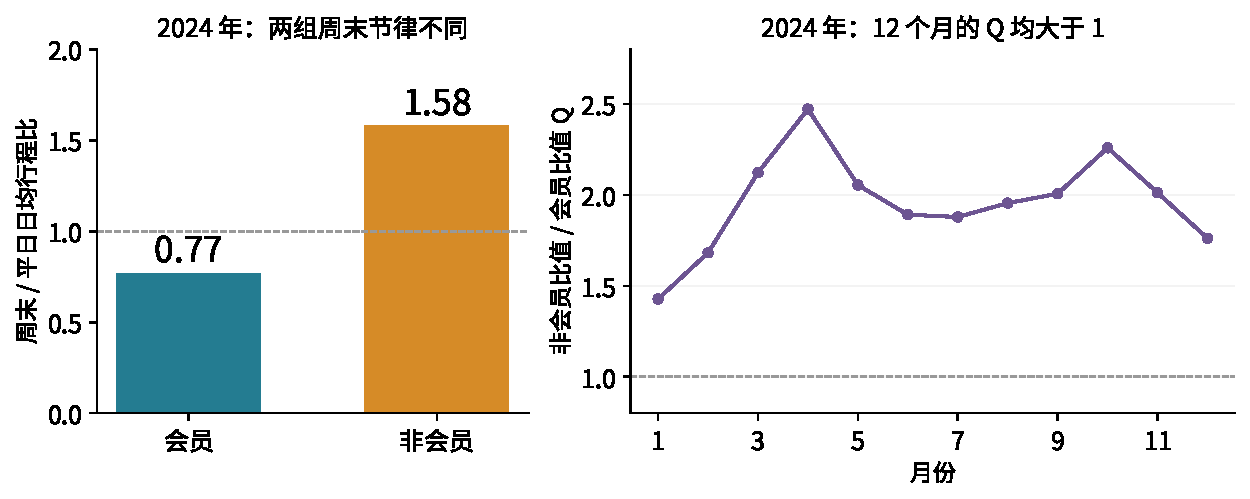
\includegraphics[width=\linewidth,height=0.65\textheight,keepaspectratio]{discovery.pdf}
  \begin{block}{选定研究问题}
    非会员的“周末日均量 / 平日日均量”是否高于会员？
  \end{block}
\end{frame}

\begin{frame}{先固定指标与验证规则}
  \[
    R_g=\frac{\text{本组周末日均行程数}}{\text{本组平日日均行程数}},
    \qquad Q=\frac{R_{\mathrm{casual}}}{R_{\mathrm{member}}},\quad H_1:Q>1.
  \]
  \begin{columns}[T,onlytextwidth]
    \begin{column}{0.47\textwidth}
      \begin{block}{全年主验证：2025 年}
        \small
        \begin{itemize}
          \item 周六、日为周末；平日含节假日。
          \item 两组配对抽取自然周块，按月份分层，重抽样 10,000 次。
          \item $Q>1$ 且 95\% 近似稳定性区间下界 $>1$：初步支持。
        \end{itemize}
      \end{block}
    \end{column}
    \begin{column}{0.49\textwidth}
      \begin{block}{额外实验：月份与天气分层}
        \small
        \begin{itemize}
          \item 月份 $\times$ 10\,$^\circ$C $\times$ 三类降水。
          \item 每格至少 2 个周末日、2 个平日。
          \item 按日期数加权汇总格内 $Q$，只作方向稳健性描述。
        \end{itemize}
      \end{block}
    \end{column}
  \end{columns}
\end{frame}

\begin{frame}{图 2：2025 年获得初步支持，天气分层后方向一致}
  \centering
  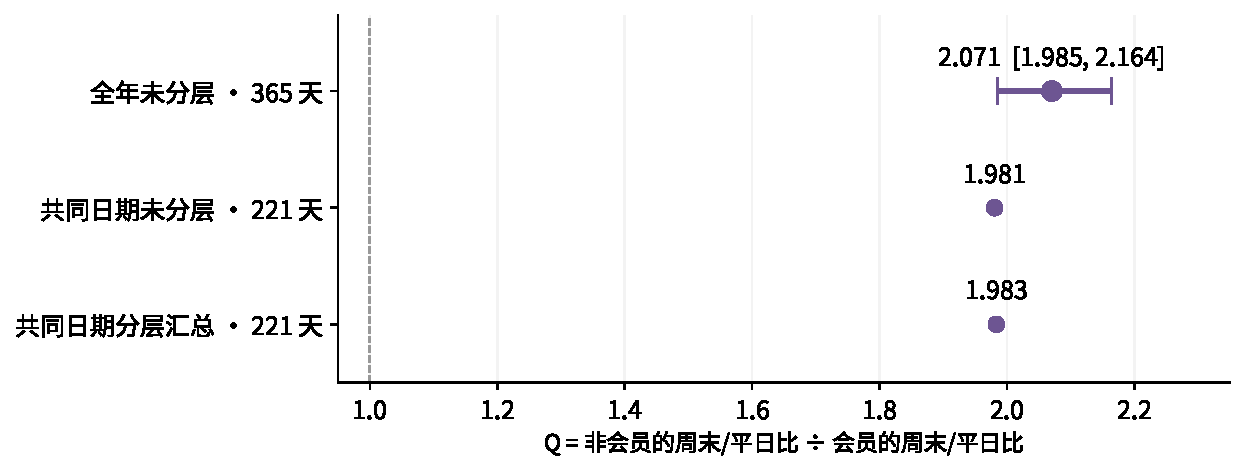
\includegraphics[width=\linewidth,height=0.66\textheight,keepaspectratio]{validation.pdf}
  \vspace{0.2em}

  \small 额外实验：27 个支持格，221 天（60.5\%），覆盖 12 个月。

  \medskip
  {\scriptsize 仅全年附 95\% 近似周块稳定性区间；分层汇总为日期加权几何平均。}
\end{frame}

\begin{frame}{结论及适用范围}
  \begin{block}{主要结论}
    2025 年非会员的周末/平日比约为会员的 \alert{2.07 倍}。\\
    在月份与天气共同支持范围内，分层汇总 $Q=1.983$，方向一致。
  \end{block}
  \begin{itemize}
    \item 结论针对既定筛选行程；站点完整性筛选明显改变车型构成。
    \item 稳定性区间依赖周块近似假设；分层仅覆盖全年 60.5\% 日期。
    \item 机场单站天气、假日及运营变化仍可能影响结果。
  \end{itemize}
\end{frame}

\begin{frame}{AI 辅助与人的研究判断}
  \begin{columns}[T,onlytextwidth]
    \begin{column}{0.48\textwidth}
      \begin{block}{AI 辅助完成}
        \begin{itemize}
          \item 下载、清洗、分析代码与测试。
          \item 发现统计线索，提出三个候选问题。
          \item 拟定验证细节，计算与制图。
          \item 整理报告与汇报材料。
        \end{itemize}
      \end{block}
    \end{column}
    \begin{column}{0.48\textwidth}
      \begin{block}{本人实际作出的判断}
        \begin{itemize}
          \item 确认数据范围与清洗口径。
          \item 确定发现年和验证年。
          \item 选择问题 A 与天气分层粒度。
          \item 审阅 PR，调整报告与汇报表述。
        \end{itemize}
      \end{block}
    \end{column}
  \end{columns}
  \medskip
  {\scriptsize 数据来源：Divvy System Data；NOAA GHCN-Daily（USW00094846）。\\
  代码、配置和运行记录：\url{https://github.com/AlphaSpire8/vibe_coding_homework}}
\end{frame}

\end{document}
